% ============================================================
% 9  Two impurities
% ============================================================
\begin{frame}
\ft{Two impurities: the RKKY sign follows the sublattice}
\begin{columns}[T]
\begin{column}{0.58\textwidth}
\[ H=\sum_{\mathbf k}\epsilon_{\mathbf k}c^\dagger_{\mathbf k}c_{\mathbf k}+J\sum_{i=1,2}\mathbf S_i\!\cdot\!\boldsymbol\sigma(\mathbf r_i) \]
\vspace{-0.1cm}
\begin{itemize}
 \item Same sublattice: \textcolor{cFM}{\textbf{FM}}
 \item Opposite sublattice: \textcolor{cAFM}{\textbf{AFM}}
 \item $J_{\rm RKKY}\propto J^2$, $T_K\sim e^{-1/J}$
\end{itemize}
\vspace{0.2cm}
\centering\footnotesize
\begin{tabular}{l|l}
\hline pair & competing regimes\\ \hline
A2--A2 & \textcolor{cFM}{FM} / \textcolor{cLM}{LM}\\
A2--B1 & \textcolor{cAFM}{AFM} / \textcolor{cLM}{LM}\\
A1--B2 & \textcolor{cAFM}{AFM} / \textcolor{cKondo}{Kondo}\\
B2--B2 & \textcolor{cFM}{FM} / \textcolor{cKondo}{Kondo}\\ \hline
\end{tabular}
\end{column}
\begin{column}{0.4\textwidth}
\centering\sitemap[0.9]{2}\\[2pt]
\legend{2}
\end{column}
\end{columns}
\tk{Only A1--B2 and B2--B2 have a nontrivial RKKY--Kondo competition}
\end{frame}
% Notes: - Two spins S_i coupled to the BLG bath with exchange J; indirect exchange J_RKKY from the nonlocal DoS.
% - Sign rule: same sublattice FM, opposite AFM (BLG is not exactly particle-hole symmetric but the asymmetry is weak).
% - A2-A2 and A2-B1 are trivial: single-impurity Kondo is absent so they just lock FM / AFM in the LM regime.
% - Map: first pair colouring appears: the A1-B2 AFM link.

% ============================================================
% 10  A1-B2 entropy
% ============================================================
\begin{frame}
\ft{A1--B2: an AFM singlet at weak $J$ crosses over to Kondo screening}
\begin{columns}[T]
\begin{column}{0.64\textwidth}
\centering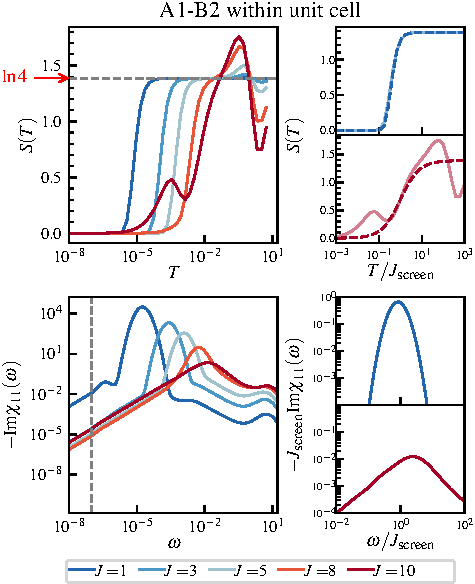
\includegraphics[height=6.7cm]{figures/split_CombFigr_0site2r0_grid.pdf}
\end{column}
\begin{column}{0.34\textwidth}
\begin{itemize}\small
 \item Weak $J$: entropy $\ln4\to0$ via $\ln2$, effective two-spin model $J_{\rm RKKY}\mathbf S_1\!\cdot\!\mathbf S_2$
 \item Strong $J$: two independent Kondo screenings
 \item Both limits follow universal curves
\end{itemize}
\end{column}
\end{columns}
\tk{Antiferromagnetic locking and Kondo screening compete at one scale}
\end{frame}
% Notes: - Top left: S(T) for several J; side panels: fits of S vs T/J_screen to the universal two-spin curves (App B).
% - Bottom: chi(omega): at weak coupling a sharp excitation at J_RKKY (singlet-triplet), at strong coupling a broad Kondo peak.
% - J_screen defined via S(J_screen)=1 (operational scale).

% ============================================================
% 11  J_screen vs J
% ============================================================
\begin{frame}
\ft{The screening scale goes from $J^2$ (RKKY) to $e^{-1/J}$ (Kondo)}
\begin{columns}[T]
\begin{column}{0.62\textwidth}
\centering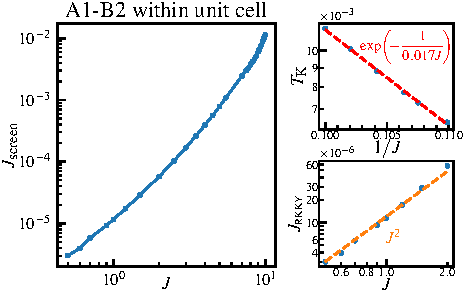
\includegraphics[width=\linewidth]{figures/AFM_scalingwithJ0v4.pdf}
\end{column}
\begin{column}{0.36\textwidth}
\begin{itemize}
 \item Weak $J$: $J_{\rm screen}\propto J^2$
 \item Strong $J$: $\propto e^{-1/J}$
 \item Insets confirm both laws
\end{itemize}
\end{column}
\end{columns}
\tk{Same configuration, two regimes: the competition is non-perturbative}
\end{frame}
% Notes: - Main panel: J_screen vs J extracted from thermodynamics (S = 1 criterion).
% - Insets: J_screen vs J^2 at weak coupling; T_K vs 1/J (log scale) at strong coupling -> single-impurity Kondo.

% ============================================================
% 12  distance
% ============================================================
\begin{frame}
\ft{The distance dependence flattens from $-1.14$ to $-0.21$ with coupling}
\begin{columns}[T]
\begin{column}{0.62\textwidth}
\centering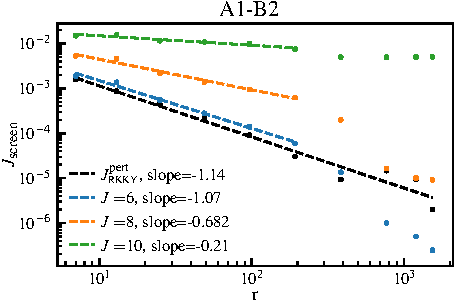
\includegraphics[width=\linewidth]{figures/JvsrSiteAFM.pdf}
\end{column}
\begin{column}{0.36\textwidth}
\begin{itemize}
 \item Perturbative RKKY: slope $-1.14$
 \item $J=10$: slope $-0.21$
 \item Strong coupling approaches the dilute Kondo limit
\end{itemize}
\end{column}
\end{columns}
\tk{At strong coupling the impurities barely feel each other}
\end{frame}
% Notes: - J_screen vs separation r (log-log) for A1-B2 pairs. Slopes: -1.14 (RKKY), -1.07, -0.682, -0.21 at J=10.
% - Optional slide: cut first if over time (move to backup).

